\documentclass[sigconf,nonacm]{acmart}
\usepackage{amsmath,booktabs,graphicx,listings}
\settopmatter{printacmref=false,printccs=false,printfolios=true}
\acmConference{}{}{}
\acmBooktitle{}
\acmYear{2026}
\copyrightyear{2026}
\setcopyright{none}
\hypersetup{hidelinks,pdftitle={Semantic Independence Coverage for JSON Schema: A Bounded Reproducible Study},pdfauthor={Sri Hari Haran Sharma}}
\lstset{basicstyle=\ttfamily\scriptsize,breaklines=true,breakatwhitespace=false,columns=fullflexible,frame=single,keepspaces=true,showstringspaces=false}
\setlength{\emergencystretch}{2em}
\renewcommand{\dbltopfraction}{.95}
\renewcommand{\dblfloatpagefraction}{.7}
\renewcommand{\textfraction}{.05}
\title{Semantic Independence Coverage for JSON Schema}
\subtitle{A Bounded Reproducible Study}
\author{Sri Hari Haran Sharma}
\email{hariharansharma588@gmail.com}
\renewcommand{\shortauthors}{Sharma}
\begin{document}
\begin{abstract}
JSON Schema validation returns a Boolean result, but a useful test suite must do more than contain accepted and rejected examples. This study operationalizes a strict semantic unique-cause criterion for explicitly selected local decisions in an annotation-free fragment of JSON Schema Draft 2020-12. The criterion belongs to the established unique-cause MC/DC and restricted active-clause family; the contribution is a scoped schema adaptation and an auditable artifact, not the invention of a new Boolean coverage principle. We express child predicates as accepted-instance sets, characterize witnesses by adjacent realizable membership cells, preserve both concrete endpoints, and distinguish finite-pool absence from unknown all-JSON feasibility. Counterexamples explain why coupled predicates, exactly-one overlap, type applicability, local-versus-root influence, and annotation-sensitive contexts defeat naive keyword-bit or union-only interpretations. The implementation separates a custom evaluator from an independently configured validator, then adds deterministic candidate generation and pair-aware suite reduction. A reproducible pilot compares decision-, predicate-, and pair-guided offline selectors with boundary-first and random selection under equal distinct-input budgets. In a 32-subject pilot, pair-aware reduction retained all 50 pool-witnessed obligations while reducing 451 candidates to 64 tests on the 21 target-bearing subjects. At an eight-test budget, pair-guided selection reached all witnessed pair targets, but its macro pool-distinguishable mutation coverage was 76.63 percent, below boundary-first selection at 91.86 percent and random selection at 77.59 percent. The paper reports this negative effectiveness result rather than claiming full-draft coverage, global feasibility, certification, first-ever novelty, or superiority at finding real faults.

\end{abstract}
\maketitle
\section{Introduction}
Suppose a schema accepts an adult age and rejects a minor age. Those two examples establish that the overall decision has both outcomes. They do not establish that every selected constraint can independently change the decision. A schema may contain redundant limits, mutually dependent alternatives, conditions that are irrelevant to the root result, or annotation effects that cannot be reconstructed from isolated truth values. A coverage report that hides these distinctions can display a reassuring percentage while omitting the evidence the percentage is intended to summarize.

The project began with two questions: can modified condition/decision coverage inform JSON Schema testing, and can sets replace an overly simple Boolean interpretation? The answer is qualified. Sets provide an established mathematical language for accepted instances; semantic condition outcomes are still Boolean observations of membership in those sets. Independence is not a third kind of truth value or the existence of one exclusive instance. It is evidence about a pair of concrete inputs under a declared decomposition and evaluation contract. The engineering task is to retain that evidence without inventing impossible truth vectors or silently treating unsuccessful search as a proof of impossibility.

We investigate four research questions. RQ1 asks whether the admitted evaluator, observations, and replayed pairs agree with a pinned independent validator on the recorded cases. RQ2 asks how much a generated finite pool can be reduced while retaining the pool's witnessed independence obligations. RQ3 asks how coverage-guided, boundary-first, and random offline choices compare at the same distinct-input budget, including a separate root-observable mutation measure. RQ4 asks which limitations remain visible: no-witness obligations, zero-obligation subjects, unsupported semantics, and mutants indistinguishable on the particular pool.

These questions separate three claims often conflated in coverage projects. An algebraic identity can be valid without yielding a complete witness solver. A reducer can preserve its selected coverage criterion without finding a minimum suite. A suite can achieve high local coverage without exposing more root-level faults. We evaluate these layers separately. The central artifact is therefore a chain from a declared schema and candidate pool to observations, eligible pairs, a selected suite, independent replay, and a report whose domain and limitations travel with its score.

The intended reader can follow the narrative without reading the code. Sections 2 and 3 explain the established background and the semantic boundaries. Sections 4 and 5 give the formal model and algorithms. Sections 6 and 7 describe the executed study and results. The appendices provide worked examples, commands, a project history, and a guide to the repository. A reader implementing or auditing the method should also inspect the source and machine-readable evidence; the prose is not a replacement for those artifacts.

\section{Background and related work}
MC/DC is a family of structural testing criteria rather than one software package. NASA's public tutorial distinguishes unique-cause and masking interpretations, discusses coupled condition occurrences, and places structural coverage beside requirements-based testing. It is historical guidance, not a verified account of current certification obligations. Our criterion deliberately omits program entry/exit coverage and makes no claim that a schema interpreter executed a particular source branch. It measures selected semantic decisions. \cite{ref1}

Logic coverage literature already formalizes active clauses, Boolean determination, and the relation between the major clause and fixed minor-clause outcomes. Under restricted active-clause coverage, the target clause changes while the other selected clause values remain equal and the predicate changes. This is the same-minor-values principle used here over feasible schema instances. Naming the relation semantic unique-cause coverage describes its application; it does not establish a new Boolean coverage criterion. Condition occurrences also require care: this artifact preserves distinct immediate child occurrences and represents equality between them through realizability, rather than silently merging repeated schema text into one coordinate. \cite{ref3}

Pair-aware reduction is also established. Jones and Harrold explicitly distinguish MC/DC's paired requirements from ordinary single-entity coverage and study build-up and break-down reduction. Their work explains why opposite condition truth values need not form a compatible independence pair. Our finite-pool optimization model and greedy implementation adapt that paired-evidence requirement to schema observations; they are not a discovery that both endpoints matter. \cite{ref2}

JSON Schema itself has substantial formal foundations. Pezoa and colleagues formalize classical syntax and semantics; subsequent work develops algebraic operators, negation elimination, and constructive witnesses. Attouche and colleagues evaluate a much broader witness-generation approach on collections that include real schemas. Modern JSON Schema has dedicated formalizations of annotation-dependent validation and dynamic references. Recent work further establishes annotation elimination, including a worst-case succinctness cost. Consequently, a counterexample to substituting standalone acceptance-equivalent fragments does not prove that a whole modern schema can never be transformed into a richer classical representation. \cite{ref4,ref5,ref6,ref7,ref8}

Existing tools are relevant comparisons, not interchangeable competitors. Hyperjump's schema-coverage project maps keywords, true/false outcomes, and subschema observations into Istanbul-style reports. It is direct evidence that JSON Schema coverage predates this artifact. Hypothesis-jsonschema generates allowed values through a strategy interface, with its inspected README stating a particular tested dialect scope. Bowtie coordinates validators and publishes comparison results. JSON subschema checking addresses containment and compatibility between accepted-value sets. These objectives differ from preserving strict semantic independence pairs. None of these tools was run as a performance competitor in this pilot, so our in-project random baseline must not be presented as an experimental comparison with them. \cite{ref11,ref12,ref13,ref20}

The defensible contribution is thus an explicit, executable contract for a bounded schema fragment: stable local occurrence identities; realizable paired observations; exact JSON numeric/equality handling; conservative unknown, unsupported, and finite-domain statuses; independent replay; and an exploratory comparison whose raw evidence can be inspected. The literature search was targeted rather than systematic. It does not establish that this exact combination is first, and this manuscript does not make that claim. Its suitability as a publishable research contribution requires the author's scholarly assessment beyond successful execution of an artifact.

\section{Semantics and scope}
Let $\mathcal{J}$ denote finite JSON values under the JSON Schema instance data model. An evaluation contract $E$ fixes the dialect, supported vocabulary and extension policy, registry and base-URI behavior, format policy, and numerical interpretation. At a schema occurrence, a context $\kappa$ additionally fixes the instance location and relevant evaluation or reference scope. Assuming a well-formed schema, resolved resources, supported semantics, and completed evaluation, define its accepted set by

\[
\begin{aligned}\mathcal{A}_{E,\kappa}(S)=\{x\in\mathcal{J}:{}&S\text{ validates }x\\&\text{under }E,\kappa\}.\end{aligned}
\]
For a fixed root contract the context subscript can be suppressed. This is an extensional projection onto validity, not a complete operational semantics. It does not encode annotations, evaluated property/index locations, error messages, branch visits, or implementation control flow. An invalid schema or unresolved evaluation is not the Boolean schema \texttt{f\allowbreak{}a\allowbreak{}l\allowbreak{}s\allowbreak{}e}; it is an input or evaluation failure. Core and Validation define these semantic categories separately. \cite{ref9,ref10}

At a common instance location and compatible fixed context, logical applicators have the familiar membership interpretation. If $A_i$ is the accepted set of child occurrence $i$, then \texttt{a\allowbreak{}l\allowbreak{}l\allowbreak{}O\allowbreak{}f} denotes $\bigcap_i A_i$, \texttt{a\allowbreak{}n\allowbreak{}y\allowbreak{}O\allowbreak{}f} denotes $\bigcup_i A_i$, and \texttt{n\allowbreak{}o\allowbreak{}t} denotes $\mathcal{J}\setminus A_1$. Exactly-one is

\[
\operatorname{One}(A_1,\ldots,A_n)
=\bigcup_i\left(A_i\setminus\bigcup_{j\ne i}A_j\right).
\]
The identity follows by replacing membership with its indicator: all, at least one, negation, and exactly one respectively recover the specification's assertion conditions. Binary \texttt{o\allowbreak{}n\allowbreak{}e\allowbreak{}O\allowbreak{}f} equals symmetric difference, but repeated symmetric difference for three or more operands means parity. With three \texttt{t\allowbreak{}r\allowbreak{}u\allowbreak{}e} children, exactly-one accepts no value whereas odd parity accepts every value. Union alone is monotone in its operands and cannot supply the complete behavior of complement or exactly-one without additional operations or encodings. These are elementary reformulations of established semantics, not new set algebra. \cite{ref5,ref6,ref9}

Type applicability is equally important. \texttt{\{\allowbreak{}"\allowbreak{}m\allowbreak{}i\allowbreak{}n\allowbreak{}i\allowbreak{}m\allowbreak{}u\allowbreak{}m\allowbreak{}"\allowbreak{}:\allowbreak{}1\allowbreak{}8\allowbreak{}\}} accepts nonnumbers as well as numbers at least 18. Adding \texttt{\{\allowbreak{}"\allowbreak{}t\allowbreak{}y\allowbreak{}p\allowbreak{}e\allowbreak{}"\allowbreak{}:\allowbreak{}"\allowbreak{}i\allowbreak{}n\allowbreak{}t\allowbreak{}e\allowbreak{}g\allowbreak{}e\allowbreak{}r\allowbreak{}"\allowbreak{}\}} excludes those nonnumbers and nonintegral numbers. A string can therefore make the selected integer predicate false while the minimum predicate remains true. Treating every keyword as a freely assigned Boolean bit invents combinations when predicates are coupled and misses vacuous success outside a keyword's target type. The specification's instance equality also distinguishes Boolean values from numbers and treats integer-valued numeric representations consistently; a host-language shortcut in which \texttt{t\allowbreak{}r\allowbreak{}u\allowbreak{}e\allowbreak{} \allowbreak{}=\allowbreak{}=\allowbreak{} \allowbreak{}1} is unsuitable. \cite{ref10}

Plain accepted sets do not support unrestricted contextual substitution. Consider $A$ equal to \texttt{\{\allowbreak{}"\allowbreak{}p\allowbreak{}r\allowbreak{}o\allowbreak{}p\allowbreak{}e\allowbreak{}r\allowbreak{}t\allowbreak{}i\allowbreak{}e\allowbreak{}s\allowbreak{}"\allowbreak{}:\allowbreak{}\{\allowbreak{}"\allowbreak{}p\allowbreak{}"\allowbreak{}:\allowbreak{}t\allowbreak{}r\allowbreak{}u\allowbreak{}e\allowbreak{}\}\allowbreak{}\}} and $B$ equal to Boolean \texttt{t\allowbreak{}r\allowbreak{}u\allowbreak{}e}. Standalone, both accept every value. Put either in \texttt{\{\allowbreak{}"\allowbreak{}a\allowbreak{}l\allowbreak{}l\allowbreak{}O\allowbreak{}f\allowbreak{}"\allowbreak{}:\allowbreak{}[\allowbreak{}H\allowbreak{}O\allowbreak{}L\allowbreak{}E\allowbreak{}]\allowbreak{},\allowbreak{}"\allowbreak{}u\allowbreak{}n\allowbreak{}e\allowbreak{}v\allowbreak{}a\allowbreak{}l\allowbreak{}u\allowbreak{}a\allowbreak{}t\allowbreak{}e\allowbreak{}d\allowbreak{}P\allowbreak{}r\allowbreak{}o\allowbreak{}p\allowbreak{}e\allowbreak{}r\allowbreak{}t\allowbreak{}i\allowbreak{}e\allowbreak{}s\allowbreak{}"\allowbreak{}:\allowbreak{}f\allowbreak{}a\allowbreak{}l\allowbreak{}s\allowbreak{}e\allowbreak{}\}} and evaluate \texttt{\{\allowbreak{}"\allowbreak{}p\allowbreak{}"\allowbreak{}:\allowbreak{}1\allowbreak{}\}}. The context with $A$ accepts because its property evaluation supplies the relevant credit; the context with $B$ rejects. Acceptance equality is therefore not a congruence for this arbitrary composition context. Likewise, all successful \texttt{a\allowbreak{}n\allowbreak{}y\allowbreak{}O\allowbreak{}f} branches can contribute evaluated-property information, so choosing only the first successful branch changes some enclosing results. \cite{ref9}

This example limits a particular abstraction, not the power of mathematical sets or compilation. Richer sets of evaluation states, relations carrying evaluated locations, or established annotation-elimination transformations can address information lost by standalone accepted-value projections. Dynamic references and recursion introduce additional context and termination questions. We use annotation-sensitive cases as independently validated explanatory fixtures, while explicitly excluding them from the coverage analyzer. This is a supported-scope decision, not a claim that the excluded semantics are impossible to model. \cite{ref7,ref8}

The implemented \texttt{p\allowbreak{}u\allowbreak{}r\allowbreak{}e\allowbreak{}-\allowbreak{}v\allowbreak{}1} fragment admits Boolean schemas, empty objects, \texttt{t\allowbreak{}y\allowbreak{}p\allowbreak{}e} including type arrays, \texttt{c\allowbreak{}o\allowbreak{}n\allowbreak{}s\allowbreak{}t}, \texttt{e\allowbreak{}n\allowbreak{}u\allowbreak{}m}, four inclusive/exclusive numeric bounds, and nested \texttt{a\allowbreak{}l\allowbreak{}l\allowbreak{}O\allowbreak{}f}, \texttt{a\allowbreak{}n\allowbreak{}y\allowbreak{}O\allowbreak{}f}, \texttt{o\allowbreak{}n\allowbreak{}e\allowbreak{}O\allowbreak{}f}, and \texttt{n\allowbreak{}o\allowbreak{}t}. It recognizes Draft 2020-12 declarations and inert title, description, and comment metadata. It rejects structural object/array/string constraints, conditionals, references, custom vocabularies, formats, \texttt{m\allowbreak{}u\allowbreak{}l\allowbreak{}t\allowbreak{}i\allowbreak{}p\allowbreak{}l\allowbreak{}e\allowbreak{}O\allowbreak{}f}, and annotation-sensitive applicators. Values of array or object type can still appear as type representatives or equality literals; that does not imply support for their structural keywords.

\section{Semantic independence coverage}
Fix one local decision occurrence, ordered selected condition occurrences $P_1,\ldots,P_n$, and its Boolean function $f$. For each admitted concrete input $x$, let $v(x)$ be the vector of child assertion outcomes and require the selected decision to satisfy $D(x)=f(v(x))$. Immediate logical children form the prototype's decomposition. Atomic sibling constraints affect root validity but do not become extra invented coordinates. A different decomposition changes the metric and its denominator and must be reported.

For each Boolean vector $b\in\{0,1\}^n$, define the membership cell

\[
R_b=\bigcap_{i=1}^n B_i(b_i),\qquad
B_i(1)=A_i,\quad B_i(0)=\mathcal{J}\setminus A_i.
\]
The nonempty cells partition the admitted domain. Every input has exactly one membership vector, placing it in one cell; distinct vectors disagree in a coordinate and hence their cells are disjoint. Some abstract vectors have empty cells. For duplicate integer branches under \texttt{a\allowbreak{}n\allowbreak{}y\allowbreak{}O\allowbreak{}f}, only vectors 00 and 11 are realizable; 01 and 10 are not missing tests but impossible combinations under that decomposition.

The strict witness relation for target coordinate $i$ is

\[
\begin{aligned}
W_i=\{\{x,y\}:&\ v_i(x)\ne v_i(y),\ D(x)\ne D(y),\\
&v_j(x)=v_j(y)\text{ for every }j\ne i\}.
\end{aligned}
\]
Both observations must refer to the same occurrence and compatible context class and have completed semantic evaluation. Input fields themselves need not remain fixed: several JSON fields can change as long as the other selected predicate outcomes do not. Conversely, changing one field is insufficient if it changes several selected predicates. This is independence relative to a declared abstraction, not a causal intervention claim about arbitrary input features.

\textbf{Proposition 1 (realizable adjacency).} A target has a witness if and only if there is a vector $b$ such that $R_b$ and $R_{b\oplus e_i}$ are both nonempty and $f(b)\ne f(b\oplus e_i)$. A concrete pair yields the two adjacent cells. Conversely, selecting one member of each nonempty adjacent cell yields a pair satisfying the relation. The proposition is a direct membership characterization of established unique-cause reasoning; it does not provide a decision procedure for either cell's nonemptiness. Boolean sensitivity on abstract vectors is insufficient unless both endpoints are realizable. \cite{ref1,ref3}

For conjunction, let $P=\bigcap_j A_j$ and $N_i=(\bigcap_{j\ne i}A_j)\setminus A_i$. A strict pair exists exactly when both $P$ and $N_i$ are nonempty. One negative exclusive point is insufficient without a positive decision witness. For disjunction, both the all-false region $Z=\mathcal{J}\setminus\bigcup_j A_j$ and exclusive region $U_i=A_i\setminus\bigcup_{j\ne i}A_j$ must be nonempty. For exactly-one, toggling $i$ changes the result only when the other coordinates contain zero or one true result; both endpoints must still be realizable.

For a suite $T$, let $C(T)=\{i:W_i\cap {T\choose2}\ne\varnothing\}$. Adding tests is monotone: $C(T)\subseteq C(T\cup U)$. However, $C(T\cup U)$ can strictly exceed $C(T)\cup C(U)$ because a compatible pair can straddle the two suites. Consequently, merging only already-covered condition IDs loses evidence that appears when runs are combined. Retaining vectors and endpoint identity is necessary for correct aggregation. This paired-requirement issue is established in MC/DC reduction literature and becomes a concrete report-design requirement here. \cite{ref2}

The usual $n+1$ intuition also needs scope. If a suite covers $n$ distinct coordinates by strict unique-cause pairs, choose one witness edge per coordinate in the Boolean cube. The selected edges have distinct coordinate labels and cannot contain a cycle: every used coordinate on a cube cycle must be flipped an even number of times. They form a forest with $n$ edges and at least $n+1$ distinct vertices. A conjunction attains the bound. This gives a lower bound under the stated total-vector model; it neither establishes feasibility nor promises an $n+1$ suite for arbitrary coupled schema predicates. It is not a masking theorem.

The report separates \texttt{c\allowbreak{}o\allowbreak{}v\allowbreak{}e\allowbreak{}r\allowbreak{}e\allowbreak{}d}, \texttt{f\allowbreak{}e\allowbreak{}a\allowbreak{}s\allowbreak{}i\allowbreak{}b\allowbreak{}l\allowbreak{}e\allowbreak{}\_\allowbreak{}u\allowbreak{}n\allowbreak{}c\allowbreak{}o\allowbreak{}v\allowbreak{}e\allowbreak{}r\allowbreak{}e\allowbreak{}d}, \texttt{p\allowbreak{}r\allowbreak{}o\allowbreak{}v\allowbreak{}e\allowbreak{}n\allowbreak{}\_\allowbreak{}i\allowbreak{}n\allowbreak{}f\allowbreak{}e\allowbreak{}a\allowbreak{}s\allowbreak{}i\allowbreak{}b\allowbreak{}l\allowbreak{}e}, \texttt{u\allowbreak{}n\allowbreak{}k\allowbreak{}n\allowbreak{}o\allowbreak{}w\allowbreak{}n}, and \texttt{u\allowbreak{}n\allowbreak{}s\allowbreak{}u\allowbreak{}p\allowbreak{}p\allowbreak{}o\allowbreak{}r\allowbreak{}t\allowbreak{}e\allowbreak{}d}. A candidate-only pair is feasible but uncovered by the selected suite. Exhaustive absence in an explicitly declared finite pool proves only pool-relative infeasibility. In all-JSON mode, unsuccessful finite search remains unknown. Invalid inputs and evaluation failures abort analysis rather than becoming false observations. Whole-schema unsupported analysis yields no fabricated complete catalog or score.

For a complete fixed catalog $O$, the conservative raw score is $|C(T)|/|O|$. A separately labeled feasibility-adjusted score can exclude only obligations proved infeasible in the score's own universe. Unknown obligations remain visible. Zero denominators are N/A rather than 100 percent. Constant and atomic schemas therefore remain useful validity subjects even though they have no invented logical independence obligations.

\section{Algorithms and implementation}
The implementation has separate ownership boundaries. Strict JSON handling owns parsing, equality, canonical serialization, and digests. A custom pure-fragment evaluator owns child outcomes and local/root validity. An oracle adapter uses a pinned \texttt{D\allowbreak{}r\allowbreak{}a\allowbreak{}f\allowbreak{}t\allowbreak{}2\allowbreak{}0\allowbreak{}2\allowbreak{}0\allowbreak{}1\allowbreak{}2\allowbreak{}V\allowbreak{}a\allowbreak{}l\allowbreak{}i\allowbreak{}d\allowbreak{}a\allowbreak{}t\allowbreak{}o\allowbreak{}r} with format assertion disabled and remote resource retrieval denied. Observation collection checks each root, each relevant child, and each local applicator against the oracle. The pair engine operates on those agreed observations, and replay reconstructs the report and compares its complete evidence rather than trusting a percentage. \cite{ref19}

Numeric input tokens are parsed exactly as decimals or integers, not rounded through binary floating point. Recursive equality distinguishes booleans before numbers. At the stock oracle boundary, integral decimals are converted exactly to integers, while nonintegral decimals remain exact decimals; this accommodates integer classification without replacing the oracle's assertion algorithms. Project canonical JSON sorts object keys and normalizes decimal coefficient/exponent representation without arithmetic-context rounding. It is explicitly a project serialization, not a claim of RFC 8785 compatibility. Experiment manifests additionally hash original source and input bytes.

Decision identity includes a content-addressed schema resource, the logical keyword's pointer and occurrence path, and the criterion version; condition identity adds the immediate-child index. All admitted decisions evaluate the same root instance location. References and structural child locations are excluded. An extension supporting them must revisit context identity rather than silently grouping observations by repeated schema text. Replay checks complete consistency in the recorded environment; it is not a cryptographic signature or proof of historical provenance.

The deterministic generator is a transparent heuristic. It collects equality literals and numeric bounds, proposes the bounds themselves, exact offsets below and above them, floor/ceiling integer neighbors, and midpoints between consecutive bounds. It adds primitive representatives and fresh string/array/object representatives outside the finite family of literal values. Equality-aware deduplication assigns stable content IDs. Schema literals and exact bounds have first priority, neighbors and midpoints second, and primitive/fresh representatives third; deterministic canonical ordering breaks ties. The generator records the proposed and retained counts, cap, truncation, reasons, and rejected representations. No universal epsilon or all-JSON completeness theorem is claimed.

For finite-pool reduction, let $X$ be the supplied candidates and $E_i$ the eligible pairs for obligation $i$. A transparent binary model selects tests $y_x$ and pair activations $z_p$:

\[
\begin{aligned}&\min\sum_{x\in X}y_x,\\&z_{\{x,y\}}\le y_x,\quad z_{\{x,y\}}\le y_y,\\&\sum_{p\in E_i}z_p\ge1.\end{aligned}
\]
The required obligations are those witnessed in this pool; empty pair sets are classified separately. Minimizing pair count is different from minimizing distinct tests because endpoints can be shared. Treating individual endpoints as ordinary set-cover elements is unsound if one endpoint receives full independence credit. These are standard paired-coverage modeling considerations applied to the artifact's explicit observations. \cite{ref2}

The greedy reducer considers adding a pair's missing endpoints together, ranks newly completed target obligations per new distinct input, and breaks ties deterministically. It then removes selected tests whose deletion preserves the achieved target. Decision- and predicate-guided comparators instead use singleton outcome features. For pools of at most 16 candidates, exact reduction enumerates at most 65536 subsets by increasing cardinality and reports a minimum only for that finite pool and completed search. Larger pools remain heuristic. The resulting selected suite is reanalyzed and replayed before reduction adequacy is reported.

Admission limits are engineering safeguards, not schema-language semantics. The generator and selector cap candidate counts and eligible pairs; exact enumeration has a smaller pool cap. Parsing, depth, nodes, numeric representation, corpus size, and report size are bounded. Expanded observation evidence must fit the replay loader, so a report that cannot be reloaded is rejected rather than emitted as successful analysis. These limits are visible in configuration and documentation; the public commands distinguish errors from unsupported analysis.

\section{Experimental methodology}
The experimental protocol freezes each schema and candidate pool before selection. The schema/pool pair, rather than a random seed, is the experimental unit. Authored subjects exercise independent conjunction/disjunction, nested decisions, duplicated predicates, redundant bounds, contradictions, exactly-one overlap, local effects masked at the root, and zero-obligation controls. Twelve official-derived subjects supplement the twenty authored schemas: the first two admitted logical groups from each allOf/anyOf/oneOf/not file, plus the first admitted type/const/enum/Boolean group as four atomic controls. Official conformance cases are developer-authored examples, not a random or industrial sample of deployed schemas. The actual subject inventory and provenance are retained with the executed experiment, and the official-derived cases retain their immutable upstream source revision. \cite{ref18}

RQ1 is checked through custom/oracle agreement, research counterexamples, admitted official cases, and replay. The baseline implementation milestone had 86 regression tests. The completed continuation passed 105 regression tests, while the pinned validation checks passed 295 admitted official tests with 52 explicit exclusions and all 43 original research expectations through the oracle. The continuation verification outputs are preserved separately from the historical baseline. The independent finite mathematics script passed 197314 assertions across 65808 Boolean-function/realizability models. These counts are evidence for their named code/input revisions, not a proof of full-draft conformance or universal correctness.

RQ2 measures reduction separately from budgeted comparison. The target is the set of pool-witnessed independence obligations. We record pool size, selected size, achieved preservation, replay status, and any exact-search result or heuristic-only status. A zero-target subject is not discarded or scored as perfect global coverage: it requires zero tests for this specific independence target and is reported as a zero-obligation or no-witness case. Adequacy preservation is expected from a correct reducer and is not used as independent proof of fault-discovery superiority.

RQ3 uses common distinct-input budgets on the same frozen pool. Decision-guided, predicate-guided, and pair-guided greedy methods are compared with a schema-derived boundary-first ordering and random sampling without replacement. Common budgets are two, four, and eight distinct inputs, and random seeds 0 through 19 provide repeated selections within each subject. The generation cap is 48; the mutation cap is 32 per subject. If a guided criterion saturates before the comparison budget, a documented common deterministic fill rule reaches the same budget. We report actual distinct-test counts and reject a comparison that spends unequal final-suite budgets without saying so. Coverage and effectiveness can be confounded by suite size, as established empirical testing studies emphasize. \cite{ref14,ref15}

A second distinction concerns preprocessing. Guided methods consult observations of the full candidate pool. They perform offline suite selection from pre-executed candidates, not free online test generation. We therefore record generation, full-pool analysis, indexing, mutation classification, selection, and replay costs separately. Random and boundary ranking do not inherently require the same coverage preprocessing. Equal final-suite budgets support an offline selection comparison, not a claim that one method discovers faults more cheaply end to end. Timings from one machine are descriptive and are not treated as statistically significant speed differences.

Root-observable schema mutations provide an exploratory outcome separate from the selector's optimized coverage target. Predeclared operators modify admitted bounds, types, literals, logical operators, or children while preserving well-formedness and support. Each unique admitted mutant retains its operator, path, digest, and evaluation evidence. For mutant $m$, define its discrepancy set in the frozen pool by $K_m=\{x\in X:\operatorname{valid}(S,x)\ne\operatorname{valid}(m,x)\}$. A selected suite distinguishes the mutant exactly when $T\cap K_m\ne\varnothing$.

If $K_m$ is empty, the mutant is pool-indistinguishable, not proved globally equivalent. The report retains total admitted mutants, pool-distinguishable mutants, pool-indistinguishable mutants, and killed counts. A normalized ratio is labeled pool-distinguishable mutant coverage and uses only its declared finite-pool denominator; a second raw ratio uses all admitted mutants. Zero denominators are N/A. Mutation results never influence coverage-only selectors. Local activation need not propagate to the root, a distinction motivating observable MC/DC in other domains. Our root-masked subjects preserve this limitation rather than filtering it out. \cite{ref16}

The experiment does not assume that these mutations model real developer faults. Evidence connecting mutants and real faults in other software does not automatically transfer to schema authoring. Multiple syntactically different mutants can also share a pool behavior, over-weighting one pattern. Persisted discrepancy sets allow an auditor to inspect that sensitivity. There is no real-fault corpus, industrial validation, or comparator-tool execution in this study. \cite{ref17}

Random repetitions are summarized within each schema before schema-level macro aggregation. Eligible-schema counts accompany each normalized metric; N/A cases are not silently converted to ones. Raw per-schema, per-budget, and per-seed rows remain available. This small pilot uses descriptive summaries and paired differences, not a significance test that pretends seeds are independent schema subjects. The experiment can reveal a negative result: pair coverage can improve while root mutation discrepancy does not. Such a result limits the method's usefulness claim rather than invalidating the witness definition.

\section{Results}
The recorded study completed all 32 subjects and 2304 equal-budget rows. Twenty schemas were authored diagnostic subjects and twelve were official-derived. The generated pools contained 630 per-subject candidate tests in total, with sizes from 16 to 32. No pool reached the declared cap, no pool was truncated, and no numeric representation proposal was rejected. These are counts within this selected study; they do not establish generator completeness or an industrial distribution.

The catalog contained 69 local condition obligations. Fifty had concrete witnesses in their respective pools, across 21 subjects. Nineteen lacked a pair in the declared pool. Four atomic controls had no catalogued logical obligations, and seven additional logical subjects had no witnessed independence target. Keeping these cases visible prevents constant, contradictory, or coupled decisions from disappearing into a misleading 100-percent aggregate. The finite-pool status says nothing by itself about feasibility outside the pool.

For the 21 subjects with witnessed targets, greedy pair-preserving reduction retained all target obligations and independently replayed every reduced report. Their candidate counts summed to 451 and their selected counts to 64, an 85.81-percent reduction in this finite-pool target-bearing total. Selected suites had two to four tests. The eleven subjects without a witnessed independence target were retained in the inventory but excluded from this reduction ratio; otherwise their zero-test independence target would inflate the headline reduction. This is adequacy preservation for a declared target, not proof of optimality or superior fault discovery.

Table 1 reports schema-macro means at equal budgets. Independence coverage uses the 21 subjects with a nonzero pool-witnessed independence denominator. Mutation coverage uses the 31 subjects with at least one pool-distinguishable mutant. These are different eligible sets, so the two columns should not be interpreted as a subject-by-subject correlation. Random scores are averaged over twenty seeds within each schema before macro aggregation. Percentages are rounded half-up from the recorded decimal summaries only for display; raw rational numerators and denominators are preserved.

\begin{table*}[t]
\centering\small
\caption{Equal-budget schema-macro means (percent). Independence uses 21 target-bearing schemas; pool-distinguishable mutant coverage uses 31 eligible schemas. Random means average seeds within schema first.}
\begin{tabular}{rlrr}
\toprule
\shortstack{Distinct\\inputs} & Selector & \shortstack{Independence\\coverage (\%)} & \shortstack{Pool-distinguishable\\mutant coverage (\%)}\\
\midrule
2 & Decision-guided & 56.98 & 56.17 \\
2 & Predicate-guided & 33.65 & 57.23 \\
2 & Pair-guided & 56.98 & 56.17 \\
2 & Boundary-first & 13.97 & 65.11 \\
2 & Random mean & 22.26 & 46.28 \\
4 & Decision-guided & 80.63 & 63.56 \\
4 & Predicate-guided & 80.00 & 70.58 \\
4 & Pair-guided & 99.05 & 70.58 \\
4 & Boundary-first & 65.24 & 75.21 \\
4 & Random mean & 44.88 & 58.95 \\
8 & Decision-guided & 90.16 & 74.10 \\
8 & Predicate-guided & 90.48 & 76.09 \\
8 & Pair-guided & 100.00 & 76.63 \\
8 & Boundary-first & 88.73 & 91.86 \\
8 & Random mean & 69.44 & 77.59 \\
\bottomrule
\end{tabular}
\end{table*}
\IfFileExists{figures/results.pdf}{
\begin{figure*}[t]
\centering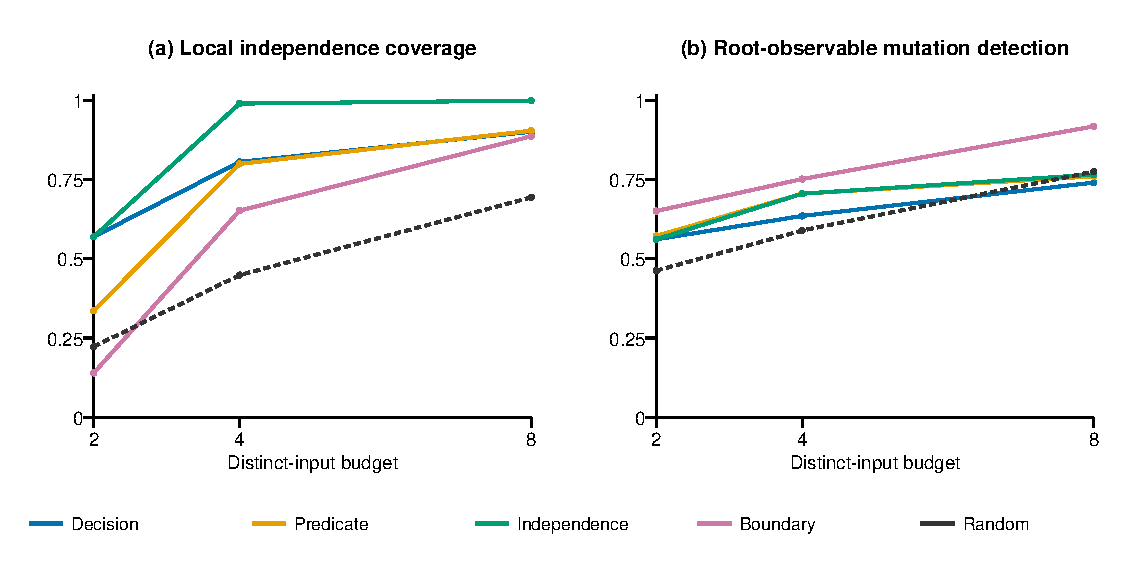
\includegraphics[width=\textwidth]{figures/results.pdf}
\caption{Coverage and root mutation outcomes are distinct. Values are descriptive schema-macro means under the frozen-pool protocol; see Table 1 for eligible denominators.}
\end{figure*}
}{}
Pair-guided selection achieved 56.98, 99.05, and 100.00 percent mean independence coverage at budgets two, four, and eight. Random selection achieved 22.26, 44.88, and 69.44 percent. As expected, an offline selector designed to complete pairs scores well on its own objective. At budget four it covered every witnessed target on 20 of 21 eligible subjects; the remaining authored nested-oneOf subject covered four of five targets. Its unconstrained reduction nevertheless ended with four tests covering all five after deletion. The contrast illustrates the myopia of the budget-constrained greedy construction, not an exact-minimum claim.

The separate mutation outcome does not show general pair-guided superiority. The study generated 177 unique admitted mutants: 139 were pool-distinguishable and 38 pool-indistinguishable. No mutation proposal was invalid or truncated in this run. At budget two, pair-guided and decision-guided selection both had 56.17-percent mean pool-distinguishable mutation coverage, compared with 65.11 percent for boundary-first and 46.28 percent for random selection. At budget four, pair-guided and predicate-guided selection tied at 70.58 percent, while boundary-first reached 75.21 percent. At budget eight, pair-guided selection reached 76.63 percent, below random's 77.59 percent and boundary-first's 91.86 percent. The negative result is central: completing local independence evidence did not make this selector best on root mutation discrepancies.

The discrepancy is consistent with the observation model. The authored masked-local subject has two witnessed local obligations, but six of its nine mutants are pool-indistinguishable at the root. The sibling-mask subject has two witnessed local obligations while seven of eight mutants are pool-indistinguishable. These cases do not invalidate local evidence; they show why propagating local variation to a root-observable effect is a separate requirement. Boundary-oriented inputs also align with the declared bound-shift mutation family, so their favorable result cannot be extrapolated to arbitrary faults or interpreted as a neutral universal winner.

Costs were recorded separately rather than hidden in final suite size. On the single tested Python 3.14.2 macOS arm64 host, median per-subject generation time was about 1.85 ms; full-pool analysis plus replay 16.02 ms; indexing 0.37 ms; mutant classification 8.23 ms; and reduction plus replay 18.24 ms. The traced Python preprocessing peak ranged from 221713 to 1367910 bytes, with median approximately 272222 bytes. This is traced allocation during the stated preprocessing region, not process resident memory or isolated selector memory. The one-run measurements are descriptive, include instrumentation overhead, and support no cross-platform speed ranking.

The manifest records the protocol, schemas, source and artifact hashes, runtime and oracle versions, and exact command \texttt{p\allowbreak{}y\allowbreak{}t\allowbreak{}h\allowbreak{}o\allowbreak{}n\allowbreak{} \allowbreak{}t\allowbreak{}o\allowbreak{}o\allowbreak{}l\allowbreak{}s\allowbreak{}/\allowbreak{}r\allowbreak{}u\allowbreak{}n\allowbreak{}\_\allowbreak{}e\allowbreak{}x\allowbreak{}p\allowbreak{}e\allowbreak{}r\allowbreak{}i\allowbreak{}m\allowbreak{}e\allowbreak{}n\allowbreak{}t\allowbreak{}s\allowbreak{}.\allowbreak{}p\allowbreak{}y}. The complete continuation verification passed 105 regression tests; its outputs are retained under \texttt{r\allowbreak{}e\allowbreak{}s\allowbreak{}u\allowbreak{}l\allowbreak{}t\allowbreak{}s\allowbreak{}/\allowbreak{}m\allowbreak{}i\allowbreak{}l\allowbreak{}e\allowbreak{}s\allowbreak{}t\allowbreak{}o\allowbreak{}n\allowbreak{}e\allowbreak{}-\allowbreak{}2\allowbreak{}/\allowbreak{}v\allowbreak{}e\allowbreak{}r\allowbreak{}i\allowbreak{}f\allowbreak{}i\allowbreak{}c\allowbreak{}a\allowbreak{}t\allowbreak{}i\allowbreak{}o\allowbreak{}n\allowbreak{}/}, leaving milestone-1 evidence intact. Per-case directories retain generated corpora and recipes, oracle-agreed pool reports, mutant schemas and discrepancy sets, reduced suites, and replay results. The aggregate table is a readable view of those artifacts, not a substitute for them. No significance test, real-fault claim, comparator-tool performance claim, global mutant equivalence conclusion, or arXiv publication status follows from these results.

\section{Threats to validity}
The first construct-validity threat is the chosen decomposition. Immediate logical children are a clear reproducible catalog, but they omit independent obligations for arbitrary atomic sibling constraints. A schema without a logical applicator has zero independence obligations even if its domain restrictions are important. The report exposes that choice; a future leaf-level or root-influence criterion would be a different metric. Runtime short-circuit conventions and masking variants are likewise outside the total semantic relation evaluated here.

The generator favors the exact families admitted by the fragment, especially numeric boundaries and equality literals. Its pool is neither exhaustive over JSON nor sampled from a universal JSON distribution. Truncation can omit a witness, and admitted numeric/depth limits constrain possible representations. A complete classical witness solver could potentially populate cells more systematically, but the artifact does not implement or claim such a solver. The distinction between finite absence and global infeasibility is therefore central, not a minor disclaimer. \cite{ref6}

The coverage-guided comparisons have an intentional objective advantage on their own metric. High pair coverage under a pair-aware selector is useful correctness/adequacy evidence, not an independent effectiveness result. The mutation outcome partly mitigates this circularity but introduces its own operator and finite-pool biases. Selection and mutation classification use the same pool. There is no held-out real-world fault distribution, and pool-indistinguishable mutants remain unresolved rather than equivalent.

Internal validity depends on the custom evaluator, oracle adapter, exact JSON representation, and analysis implementation. Their separation reduces some shared logic, but one pinned Python validator is not a formally independent proof or a multi-validator consensus. Normalization and common parsing can still introduce shared errors. Regression cases and official examples cover recorded behaviors, while replay detects inconsistent evidence and environment drift; neither guarantees arbitrary correctness. The prototype rejects unsupported whole-schema semantics to avoid presenting a misleading partial catalog as a global percentage.

External validity is limited by authored synthetic subjects, selected official schemas, one host/runtime, and a small fixed seed set. Official cases are conformance examples rather than deployed schemas. Timings include Python and oracle overhead and can be noisy. Random seeds are reproducibility parameters, not extra independent populations. No conclusions extend directly to annotations, dynamic references, regex constraints, recursive schemas, full arrays/objects, real API workloads, or compiler code coverage.

The related-work search is targeted. Existing formalization, generation, schema coverage, and MC/DC reduction substantially overlap the foundations. This paper does not establish first-ever novelty, a new coverage principle, or a new impossibility theorem about modern JSON Schema. Its contribution is the explicit bounded adaptation, auditable engineering contract, and exploratory evidence. Whether that contribution warrants scholarly publication remains for author and peer assessment.

\section{Conclusions}
A semantic independence tool should expose what is missing as carefully as what is covered. Realizability prevents impossible truth-vector credit; paired endpoints prevent one-sided evidence; context qualifications prevent local observations from being promoted into unsupported root or execution claims. These requirements make the resulting percentage less universal but its evidence more inspectable.

The practical research question remains empirical. A useful next extension is not merely a larger percentage denominator; it is an explicit observation model for the added semantics, an independently checked witness mechanism, and a fair evaluation on a broader corpus. The present artifact provides a reproducible place to ask that question while preserving finite-domain limits, negative cases, and prior-work boundaries.

\appendix
\section{Worked examples}
Consider \texttt{\{\allowbreak{}"\allowbreak{}a\allowbreak{}l\allowbreak{}l\allowbreak{}O\allowbreak{}f\allowbreak{}"\allowbreak{}:\allowbreak{}[\allowbreak{}\{\allowbreak{}"\allowbreak{}t\allowbreak{}y\allowbreak{}p\allowbreak{}e\allowbreak{}"\allowbreak{}:\allowbreak{}"\allowbreak{}i\allowbreak{}n\allowbreak{}t\allowbreak{}e\allowbreak{}g\allowbreak{}e\allowbreak{}r\allowbreak{}"\allowbreak{}\}\allowbreak{},\allowbreak{}\{\allowbreak{}"\allowbreak{}m\allowbreak{}i\allowbreak{}n\allowbreak{}i\allowbreak{}m\allowbreak{}u\allowbreak{}m\allowbreak{}"\allowbreak{}:\allowbreak{}1\allowbreak{}8\allowbreak{}\}\allowbreak{}]\allowbreak{}\}} with inputs 18, 17, and \texttt{"\allowbreak{}x\allowbreak{}"}. Their selected vectors are 11, 10, and 01 respectively. The pair 18/\texttt{"\allowbreak{}x\allowbreak{}"} witnesses the integer coordinate because minimum holds for both; the pair 18/17 witnesses minimum because both inputs are integers. These three distinct inputs cover both local independence obligations. A different suite containing only vectors 00 and 11 for an abstract conjunction would cover both condition outcomes and both decision outcomes but no strict independence pair.

For \texttt{\{\allowbreak{}"\allowbreak{}a\allowbreak{}n\allowbreak{}y\allowbreak{}O\allowbreak{}f\allowbreak{}"\allowbreak{}:\allowbreak{}[\allowbreak{}\{\allowbreak{}"\allowbreak{}t\allowbreak{}y\allowbreak{}p\allowbreak{}e\allowbreak{}"\allowbreak{}:\allowbreak{}"\allowbreak{}i\allowbreak{}n\allowbreak{}t\allowbreak{}e\allowbreak{}g\allowbreak{}e\allowbreak{}r\allowbreak{}"\allowbreak{}\}\allowbreak{},\allowbreak{}\{\allowbreak{}"\allowbreak{}t\allowbreak{}y\allowbreak{}p\allowbreak{}e\allowbreak{}"\allowbreak{}:\allowbreak{}"\allowbreak{}i\allowbreak{}n\allowbreak{}t\allowbreak{}e\allowbreak{}g\allowbreak{}e\allowbreak{}r\allowbreak{}"\allowbreak{}\}\allowbreak{}]\allowbreak{}\}}, an integer and a string produce only 11 and 00. Both predicates change together, so neither child occurrence has a strict unique-cause pair. Deduplicating the two occurrences would change the catalog and denominator, not solve the original coverage problem. The tool reports the chosen catalog rather than silently rewriting the schema.

For \texttt{\{\allowbreak{}"\allowbreak{}a\allowbreak{}l\allowbreak{}l\allowbreak{}O\allowbreak{}f\allowbreak{}"\allowbreak{}:\allowbreak{}[\allowbreak{}\{\allowbreak{}"\allowbreak{}m\allowbreak{}i\allowbreak{}n\allowbreak{}i\allowbreak{}m\allowbreak{}u\allowbreak{}m\allowbreak{}"\allowbreak{}:\allowbreak{}0\allowbreak{}\}\allowbreak{},\allowbreak{}\{\allowbreak{}"\allowbreak{}m\allowbreak{}i\allowbreak{}n\allowbreak{}i\allowbreak{}m\allowbreak{}u\allowbreak{}m\allowbreak{}"\allowbreak{}:\allowbreak{}1\allowbreak{}0\allowbreak{}\}\allowbreak{}]\allowbreak{}\}}, the weaker minimum cannot fail while the stronger one passes. Its exclusive negative region is empty. Values 5 and 10 can witness the stronger constraint, while nonnumbers satisfy both numerical assertions. An analyzer that treats the two minima as independent unconstrained bits would invent a nonexistent witness for the weaker condition.

For \texttt{\{\allowbreak{}"\allowbreak{}a\allowbreak{}l\allowbreak{}l\allowbreak{}O\allowbreak{}f\allowbreak{}"\allowbreak{}:\allowbreak{}[\allowbreak{}f\allowbreak{}a\allowbreak{}l\allowbreak{}s\allowbreak{}e\allowbreak{},\allowbreak{}\{\allowbreak{}"\allowbreak{}a\allowbreak{}n\allowbreak{}y\allowbreak{}O\allowbreak{}f\allowbreak{}"\allowbreak{}:\allowbreak{}[\allowbreak{}\{\allowbreak{}"\allowbreak{}c\allowbreak{}o\allowbreak{}n\allowbreak{}s\allowbreak{}t\allowbreak{}"\allowbreak{}:\allowbreak{}0\allowbreak{}\}\allowbreak{},\allowbreak{}\{\allowbreak{}"\allowbreak{}c\allowbreak{}o\allowbreak{}n\allowbreak{}s\allowbreak{}t\allowbreak{}"\allowbreak{}:\allowbreak{}1\allowbreak{}\}\allowbreak{}]\allowbreak{}\}\allowbreak{}]\allowbreak{}\}}, the inner decision changes between 0 and 2, yet the root remains false. A local pair is legitimate under the local catalog. It is not root influence and need not distinguish root-observable mutations. The distinction is visible in separate local and root observations rather than hidden behind one aggregate metric.

For \texttt{\{\allowbreak{}"\allowbreak{}o\allowbreak{}n\allowbreak{}e\allowbreak{}O\allowbreak{}f\allowbreak{}"\allowbreak{}:\allowbreak{}[\allowbreak{}t\allowbreak{}r\allowbreak{}u\allowbreak{}e\allowbreak{},\allowbreak{}t\allowbreak{}r\allowbreak{}u\allowbreak{}e\allowbreak{},\allowbreak{}t\allowbreak{}r\allowbreak{}u\allowbreak{}e\allowbreak{}]\allowbreak{}\}}, the root always rejects. Interpreting exactly-one as iterated XOR would instead accept every instance. This small case prevents a plausible but incorrect set transformation. It also illustrates why observing a child as true does not imply that it has decision-flipping influence.

\section{Reproducibility and artifacts}
The repository is \texttt{h\allowbreak{}t\allowbreak{}t\allowbreak{}p\allowbreak{}s\allowbreak{}:\allowbreak{}/\allowbreak{}/\allowbreak{}g\allowbreak{}i\allowbreak{}t\allowbreak{}h\allowbreak{}u\allowbreak{}b\allowbreak{}.\allowbreak{}c\allowbreak{}o\allowbreak{}m\allowbreak{}/\allowbreak{}c\allowbreak{}h\allowbreak{}a\allowbreak{}n\allowbreak{}n\allowbreak{}i\allowbreak{}2\allowbreak{}3\allowbreak{}/\allowbreak{}s\allowbreak{}c\allowbreak{}h\allowbreak{}e\allowbreak{}m\allowbreak{}a\allowbreak{}-\allowbreak{}c\allowbreak{}o\allowbreak{}v\allowbreak{}e\allowbreak{}r\allowbreak{}a\allowbreak{}g\allowbreak{}e\allowbreak{}-\allowbreak{}l\allowbreak{}a\allowbreak{}b}. Work was performed directly on \texttt{m\allowbreak{}a\allowbreak{}i\allowbreak{}n} after the author explicitly requested consolidation of the initial research PR stack. The repository preserves those issues, PRs, commits, research chapters, and evidence logs rather than deleting completed history. A source/content manifest is preferable to relying on a moving branch name when reproducing an experiment.

Read this manuscript first for the argument, then \texttt{d\allowbreak{}o\allowbreak{}c\allowbreak{}s\allowbreak{}/\allowbreak{}U\allowbreak{}S\allowbreak{}A\allowbreak{}G\allowbreak{}E\allowbreak{}.\allowbreak{}m\allowbreak{}d} for commands, \texttt{d\allowbreak{}o\allowbreak{}c\allowbreak{}s\allowbreak{}/\allowbreak{}A\allowbreak{}R\allowbreak{}C\allowbreak{}H\allowbreak{}I\allowbreak{}T\allowbreak{}E\allowbreak{}C\allowbreak{}T\allowbreak{}U\allowbreak{}R\allowbreak{}E\allowbreak{}.\allowbreak{}m\allowbreak{}d} for implementation ownership, \texttt{d\allowbreak{}o\allowbreak{}c\allowbreak{}s\allowbreak{}/\allowbreak{}S\allowbreak{}T\allowbreak{}A\allowbreak{}T\allowbreak{}U\allowbreak{}S\allowbreak{}.\allowbreak{}m\allowbreak{}d} for current completion, and \texttt{d\allowbreak{}o\allowbreak{}c\allowbreak{}s\allowbreak{}/\allowbreak{}E\allowbreak{}V\allowbreak{}I\allowbreak{}D\allowbreak{}E\allowbreak{}N\allowbreak{}C\allowbreak{}E\allowbreak{}\_\allowbreak{}L\allowbreak{}O\allowbreak{}G\allowbreak{}.\allowbreak{}m\allowbreak{}d} for the chronology. The detailed research chapters under \texttt{d\allowbreak{}o\allowbreak{}c\allowbreak{}s\allowbreak{}/\allowbreak{}r\allowbreak{}e\allowbreak{}s\allowbreak{}e\allowbreak{}a\allowbreak{}r\allowbreak{}c\allowbreak{}h\allowbreak{}/} preserve definitions, counterexamples, primary sources, and dated limitations. \texttt{C\allowbreak{}O\allowbreak{}D\allowbreak{}E\allowbreak{}X\allowbreak{}\_\allowbreak{}H\allowbreak{}A\allowbreak{}N\allowbreak{}D\allowbreak{}O\allowbreak{}F\allowbreak{}F\allowbreak{}.\allowbreak{}m\allowbreak{}d} is the engineering contract that guided the implementation. The original fixture catalogs are project-authored examples; the vendored official subset retains its upstream MIT license and immutable source commit.

From the repository root, create a virtual environment and install \texttt{r\allowbreak{}e\allowbreak{}q\allowbreak{}u\allowbreak{}i\allowbreak{}r\allowbreak{}e\allowbreak{}m\allowbreak{}e\allowbreak{}n\allowbreak{}t\allowbreak{}s\allowbreak{}.\allowbreak{}l\allowbreak{}o\allowbreak{}c\allowbreak{}k} with hash checking. The lock fixes the tested dependency resolution. Installation can require network package access; analysis, replay, and vendored tests require no remote schema retrieval. The tested baseline runtime is Python 3.14.2 on macOS arm64. Other Python/platform combinations require their own evidence; a declared compatible version range is not a claim that every combination was tested.

\begin{lstlisting}
python3 -m venv .venv
source .venv/bin/activate
python -m pip install --require-hashes -r requirements.lock
python tools/verify.py
python -m schema_coverage_lab analyze --schema examples/conjunction.schema.json --corpus examples/conjunction.instances.json --output results/example.json
python -m schema_coverage_lab replay --report results/example.json
\end{lstlisting}
The baseline verification entry point saves actual pytest, finite-mathematics, research-fixture, official-subset, example-report, and replay outputs. The continuation commands below generate a corpus, analyze and reduce it, replay the reduction, and rerun the frozen study. Generation metadata is retained with the corpus; analysis evaluates its embedded instances under the declared domain rather than trusting a completeness claim. Each manifest records commands, exit statuses, the environment, source/input hashes, and artifact hashes. The continuation verification writes its own evidence under \texttt{r\allowbreak{}e\allowbreak{}s\allowbreak{}u\allowbreak{}l\allowbreak{}t\allowbreak{}s\allowbreak{}/\allowbreak{}m\allowbreak{}i\allowbreak{}l\allowbreak{}e\allowbreak{}s\allowbreak{}t\allowbreak{}o\allowbreak{}n\allowbreak{}e\allowbreak{}-\allowbreak{}2\allowbreak{}/\allowbreak{}v\allowbreak{}e\allowbreak{}r\allowbreak{}i\allowbreak{}f\allowbreak{}i\allowbreak{}c\allowbreak{}a\allowbreak{}t\allowbreak{}i\allowbreak{}o\allowbreak{}n\allowbreak{}/} rather than rewriting the historical milestone-1 run. A new run can replace its generated continuation artifacts; a committed evidence entry identifies which run supports a claim. Replay recomputes a report and rejects mismatched evidence or configuration. It does not authenticate who produced an old file.

\begin{lstlisting}
python -m schema_coverage_lab generate --schema examples/conjunction.schema.json --max-candidates 48 --output results/generated.json
python -m schema_coverage_lab analyze --schema examples/conjunction.schema.json --corpus results/generated.json --domain candidate_pool --output results/generated-report.json
python -m schema_coverage_lab reduce --report results/generated-report.json --criterion independence --method greedy --output results/reduced.json
python -m schema_coverage_lab replay --report results/reduced.json
python tools/run_experiments.py
python tools/verify.py --output results/milestone-2/verification --evidence-id E-0003 --base-commit c48fbe4ec1aa49f0b4bd2b8eb0797944981034fa
python tools/audit_artifacts.py
\end{lstlisting}
Artifact availability is independent of a moving branch name: the public repository is \href{https://github.com/channi23/schema-coverage-lab}{Schema Coverage Lab}. The executed study input digest is \texttt{f\allowbreak{}b\allowbreak{}8\allowbreak{}9\allowbreak{}5\allowbreak{}8\allowbreak{}b\allowbreak{}9\allowbreak{}6\allowbreak{}8\allowbreak{}1\allowbreak{}d\allowbreak{}9\allowbreak{}5\allowbreak{}2\allowbreak{}2\allowbreak{}8\allowbreak{}a\allowbreak{}2\allowbreak{}c\allowbreak{}3\allowbreak{}f\allowbreak{}0\allowbreak{}c\allowbreak{}0\allowbreak{}8\allowbreak{}8\allowbreak{}6\allowbreak{}8\allowbreak{}2\allowbreak{}5\allowbreak{}d\allowbreak{}c\allowbreak{}4\allowbreak{}5\allowbreak{}a\allowbreak{}a\allowbreak{}f\allowbreak{}b\allowbreak{}5\allowbreak{}4\allowbreak{}5\allowbreak{}f\allowbreak{}f\allowbreak{}b\allowbreak{}8\allowbreak{}0\allowbreak{}8\allowbreak{}7\allowbreak{}3\allowbreak{}d\allowbreak{}8\allowbreak{}e\allowbreak{}5\allowbreak{}e\allowbreak{}3\allowbreak{}5\allowbreak{}a\allowbreak{}6\allowbreak{}6\allowbreak{}6\allowbreak{}d\allowbreak{}d\allowbreak{}c}; the final experiment source-set digest is \texttt{7\allowbreak{}4\allowbreak{}7\allowbreak{}e\allowbreak{}8\allowbreak{}9\allowbreak{}5\allowbreak{}d\allowbreak{}6\allowbreak{}f\allowbreak{}0\allowbreak{}b\allowbreak{}4\allowbreak{}3\allowbreak{}4\allowbreak{}3\allowbreak{}8\allowbreak{}7\allowbreak{}5\allowbreak{}4\allowbreak{}5\allowbreak{}9\allowbreak{}9\allowbreak{}0\allowbreak{}e\allowbreak{}2\allowbreak{}a\allowbreak{}a\allowbreak{}8\allowbreak{}8\allowbreak{}b\allowbreak{}f\allowbreak{}5\allowbreak{}8\allowbreak{}9\allowbreak{}b\allowbreak{}2\allowbreak{}0\allowbreak{}b\allowbreak{}6\allowbreak{}4\allowbreak{}6\allowbreak{}8\allowbreak{}5\allowbreak{}2\allowbreak{}c\allowbreak{}b\allowbreak{}e\allowbreak{}a\allowbreak{}0\allowbreak{}b\allowbreak{}7\allowbreak{}d\allowbreak{}5\allowbreak{}8\allowbreak{}8\allowbreak{}c\allowbreak{}5\allowbreak{}4\allowbreak{}a\allowbreak{}3\allowbreak{}1\allowbreak{}e\allowbreak{}1}. The experiment manifest defines the source-set construction and records individual SHA-256 values for code, tests, protocol, inputs, vendored files and generated outputs. These hashes identify the executed content even if main subsequently moves. The stable implementation and experiment revision is \href{https://github.com/channi23/schema-coverage-lab/commit/f9b84dc6adf5a085f8014e4619cf0eb02a74cc6d}{f9b84dc6adf5a085f8014e4619cf0eb02a74cc6d}; use that revision with the manifest for reproduction. The source archive accompanying this manuscript provides the paper separately.

The frozen protocol is \texttt{b\allowbreak{}e\allowbreak{}n\allowbreak{}c\allowbreak{}h\allowbreak{}m\allowbreak{}a\allowbreak{}r\allowbreak{}k\allowbreak{}s\allowbreak{}/\allowbreak{}R\allowbreak{}E\allowbreak{}A\allowbreak{}D\allowbreak{}M\allowbreak{}E\allowbreak{}.\allowbreak{}m\allowbreak{}d}; exact schemas and parameters are in \texttt{b\allowbreak{}e\allowbreak{}n\allowbreak{}c\allowbreak{}h\allowbreak{}m\allowbreak{}a\allowbreak{}r\allowbreak{}k\allowbreak{}s\allowbreak{}/\allowbreak{}s\allowbreak{}t\allowbreak{}u\allowbreak{}d\allowbreak{}y\allowbreak{}.\allowbreak{}j\allowbreak{}s\allowbreak{}o\allowbreak{}n}. Results are under \texttt{r\allowbreak{}e\allowbreak{}s\allowbreak{}u\allowbreak{}l\allowbreak{}t\allowbreak{}s\allowbreak{}/\allowbreak{}m\allowbreak{}i\allowbreak{}l\allowbreak{}e\allowbreak{}s\allowbreak{}t\allowbreak{}o\allowbreak{}n\allowbreak{}e\allowbreak{}-\allowbreak{}2\allowbreak{}/}: \texttt{s\allowbreak{}u\allowbreak{}m\allowbreak{}m\allowbreak{}a\allowbreak{}r\allowbreak{}y\allowbreak{}.\allowbreak{}j\allowbreak{}s\allowbreak{}o\allowbreak{}n} gives schema-macro descriptive statistics, \texttt{o\allowbreak{}b\allowbreak{}s\allowbreak{}e\allowbreak{}r\allowbreak{}v\allowbreak{}a\allowbreak{}t\allowbreak{}i\allowbreak{}o\allowbreak{}n\allowbreak{}s\allowbreak{}.\allowbreak{}j\allowbreak{}s\allowbreak{}o\allowbreak{}n} preserves all 2304 budget/seed rows, \texttt{s\allowbreak{}u\allowbreak{}b\allowbreak{}j\allowbreak{}e\allowbreak{}c\allowbreak{}t\allowbreak{}s\allowbreak{}.\allowbreak{}j\allowbreak{}s\allowbreak{}o\allowbreak{}n} records costs and provenance, and the manifest connects source/input/artifact digests. Case directories provide complete pool/reduction/mutation evidence. Engine version 0.2.0 adds these continuation features; historical version-0.1.0 reports remain evidence for their original source revision, not a promise of cross-version replay.

Command success and unsupported analysis are distinct. Exit zero means supported success, exit two an input/evaluation/replay failure, and exit three unsupported analysis. An unsupported schema receives diagnostic locations without a fabricated complete catalog or global score. A user should always inspect exit status and scope before interpreting a report. Finite-pool results are useful for the supplied pool, even when all-JSON feasibility is unknown.

\section{Project history and author review}
The initial phase researched MC/DC definitions and implementations, Draft 2020-12 semantics, accepted-set identities, counterexamples, and a Codex implementation handoff. Five stage issues and five draft PRs made the research sequence inspectable. After the user merged the first stages and requested consolidation, the remaining stages were reconciled onto \texttt{m\allowbreak{}a\allowbreak{}i\allowbreak{}n}; the completed research/handoff issues were closed while the broader implementation/testing issue remained open.

The first implementation milestone built the strict parser, exact data model, admitted evaluator, support checker, local catalog, corpus analyzer, independent oracle comparisons, and replayable reports. It saved its own verification outputs and source digests. The continuation added deterministic candidate recipes, pair-aware selection and bounded exact enumeration, then completed the 32-subject frozen-pool study. It demonstrated strong pair-coverage preservation and a mixed or negative separate mutation result, making the distinction between adequacy and effectiveness concrete. The narrative is chronological evidence of what was attempted and completed, not proof that the resulting method is universally effective.

The named author should review all mathematical statements, source attributions, code, and numerical conclusions before submission. Drafting, implementation, research coordination, and editing were assisted by an AI coding system. The author remains responsible for the manuscript's claims and any submission. No arXiv submission, endorsement, peer review, acceptance, or publication is claimed by preparing these files. No affiliation has been supplied or invented. A separate publication-review document records remaining scholarly and submission-readiness checks.

\begin{thebibliography}{99}
\small
\raggedright
\bibitem{ref1} Kelly J. Hayhurst, Dan S. Veerhusen, John J. Chilenski, and Leanna K. Rierson. A Practical Tutorial on Modified Condition/Decision Coverage. NASA/TM-2001-210876, 2001. \href{https://ntrs.nasa.gov/citations/20010057789}{Official report}.

\bibitem{ref2} James A. Jones and Mary Jean Harrold. Test-Suite Reduction and Prioritization for Modified Condition/Decision Coverage. IEEE Transactions on Software Engineering 29(3), 195-209, 2003. \href{https://bowringj.people.charleston.edu/docs/tse03-mcdc.pdf}{Original paper}.

\bibitem{ref3} Paul Ammann, Jeff Offutt, and Hong Huang. Coverage Criteria for Logical Expressions. ISSRE 2003, 99-107. DOI 10.1109/ISSRE.2003.1251034. \href{https://doi.org/10.1109/ISSRE.2003.1251034}{Publisher record}.

\bibitem{ref4} Felipe Pezoa, Juan L. Reutter, Fernando Suarez, Martin Ugarte, and Domagoj Vrgoc. Foundations of JSON Schema. WWW 2016, 263-273. DOI 10.1145/2872427.2883029. \href{https://archives.iw3c2.org/www2016/WWW2016-Proceedings/proceedings/p263.pdf}{Proceedings paper}.

\bibitem{ref5} Mohamed-Amine Baazizi, Dario Colazzo, Giorgio Ghelli, Carlo Sartiani, and Stefanie Scherzinger. Not Elimination and Witness Generation for JSON Schema. arXiv:2104.14828v2, 2021. \href{https://arxiv.org/abs/2104.14828v2}{Versioned preprint}.

\bibitem{ref6} Lyes Attouche, Mohamed-Amine Baazizi, Dario Colazzo, Giorgio Ghelli, Carlo Sartiani, and Stefanie Scherzinger. Witness Generation for JSON Schema. PVLDB 15(13), 4002-4014, 2022. DOI 10.14778/3565838.3565852. \href{https://www.vldb.org/pvldb/vol15/p4002-sartiani.pdf}{Original paper}.

\bibitem{ref7} Lyes Attouche, Mohamed-Amine Baazizi, Dario Colazzo, Giorgio Ghelli, Carlo Sartiani, and Stefanie Scherzinger. Validation of Modern JSON Schema: Formalization and Complexity. arXiv:2307.10034v2, 2024 revision. \href{https://arxiv.org/abs/2307.10034v2}{Versioned preprint}.

\bibitem{ref8} Lyes Attouche, Mohamed-Amine Baazizi, Dario Colazzo, Giorgio Ghelli, Stefan Klessinger, Carlo Sartiani, and Stefanie Scherzinger. Elimination of annotation dependencies in validation for Modern JSON Schema. Theoretical Computer Science 1063, 115645, 2026. DOI 10.1016/j.tcs.2025.115645. \href{https://arxiv.org/abs/2503.11288}{Author preprint}.

\bibitem{ref9} JSON Schema. Draft 2020-12 Core, especially Sections 7, 8.2.3, 10 and 11. \href{https://json-schema.org/draft/2020-12/json-schema-core}{Specification}. Accessed 2026-11-09.

\bibitem{ref10} JSON Schema. Draft 2020-12 Validation, especially Sections 4 and 6-9. \href{https://json-schema.org/draft/2020-12/json-schema-validation}{Specification}. Accessed 2026-11-09.

\bibitem{ref11} Hyperjump. JSON Schema Test Coverage, official repository and documentation. \href{https://github.com/hyperjump-io/json-schema-coverage/}{Project}. Accessed 2026-11-09; not experimentally benchmarked here.

\bibitem{ref12} Hypothesis. hypothesis-jsonschema, official repository and README. \href{https://github.com/python-jsonschema/hypothesis-jsonschema}{Project}. Accessed 2026-11-09; not experimentally benchmarked here.

\bibitem{ref13} Bowtie. Official documentation. \href{https://docs.bowtie.report/en/stable/}{Project documentation}. Accessed 2026-11-09; not experimentally benchmarked here.

\bibitem{ref14} Laura Inozemtseva and Reid Holmes. Coverage Is Not Strongly Correlated with Test Suite Effectiveness. ICSE 2014, 435-445. DOI 10.1145/2568225.2568271. \href{https://www.cs.ubc.ca/~rtholmes/papers/icse_2014_inozemtseva.pdf}{Author-hosted paper}.

\bibitem{ref15} Milos Gligoric, Alex Groce, Chaoqiang Zhang, Rohan Sharma, Mohammad Amin Alipour, and Darko Marinov. Guidelines for Coverage-Based Comparisons of Non-Adequate Test Suites. ACM TOSEM 24(4), article 22, 2015. \href{https://mir.cs.illinois.edu/marinov/publications/GligoricETAL15CoCoJournal.pdf}{Author-hosted manuscript}.

\bibitem{ref16} Michael W. Whalen, Gregory Gay, Dongjiang You, Mats P. E. Heimdahl, and Matt Staats. Observable Modified Condition/Decision Coverage. ICSE 2013, 102-111. DOI 10.1109/ICSE.2013.6606556. \href{https://greg4cr.github.io/pdf/13omcdc.pdf}{Author-hosted paper}.

\bibitem{ref17} Rene Just, Darioush Jalali, Laura Inozemtseva, Michael D. Ernst, Reid Holmes, and Gordon Fraser. Are mutants a valid substitute for real faults in software testing? FSE 2014, 654-665. \href{https://homes.cs.washington.edu/~mernst/pubs/mutation-effectiveness-fse2014-abstract.html}{Author publication and BibTeX}.

\bibitem{ref18} JSON Schema organization. JSON Schema Test Suite. \href{https://github.com/json-schema-org/JSON-Schema-Test-Suite}{Repository}. Artifact subset pinned to commit 245a45abc90190c0bff04d97e6d2b541b4bb9f12; upstream MIT license retained.

\bibitem{ref19} Python jsonschema. Schema Validation and JSON Referencing documentation. \href{https://python-jsonschema.readthedocs.io/en/stable/validate/}{Validation API} and \href{https://python-jsonschema.readthedocs.io/en/stable/referencing/}{referencing API}. Accessed 2026-11-09. Experimental oracle version 4.26.0.

\bibitem{ref20} Andrew Habib, Avraham Shinnar, Martin Hirzel, and Michael Pradel. Finding Data Compatibility Bugs with JSON Subschema Checking. ISSTA 2021, 620-632. DOI 10.1145/3460319.3464796. \href{https://andrewhabib.org/publications/issta21-JSONSubschema.pdf}{Author-hosted paper}.

\end{thebibliography}
\end{document}
